% small.tex
\documentclass{beamer}
\usetheme{Madrid}
\usepackage[absolute,overlay]{textpos}
\usepackage{pgfgantt}
\usepackage{mdframed}
\begin{document}

\newenvironment{footer}[2]{%
  \begin{textblock*}{\textwidth}(#1,#2)
      \footnotesize\it\bgroup\color{red!50!black}}{\egroup\end{textblock*}}

\title{Fuzzy Logic}
\subtitle{Web Based Inferencing and Visualisation}
\author[C. Knott]{Craig Knott}
\institute[cxk01u]{
  \ \\
  With supervision from Professor Jon Garibaldi
}
\date{November 27, 2013}



\begin{frame}[plain]
  \titlepage
\end{frame}

\title{}

\begin{frame}
\frametitle{What is Fuzzy Logic?}
\only<1>{}
\only<2>{
\begin{minipage}{0.75\textwidth}
	\begin{itemize}
	\item Formalised by Lotfi Zadeh in 1965.
	\end{itemize}
\end{minipage}
\begin{minipage}{0.2\textwidth}
\begin{figure}[r]
\hspace{-1cm}
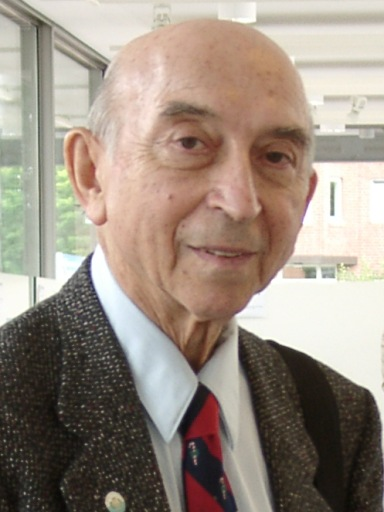
\includegraphics{images/lotfi.jpg}
\end{figure}
\end{minipage}
}
% first block disappears and the second appears
\only<3>{
\begin{minipage}{0.75\textwidth}
	\begin{itemize}
	\item Formalised by Lotfi Zadeh in 1965.
	\item No strict truth values
	\end{itemize}
\end{minipage}
}
\only<4>{
\begin{minipage}{0.75\textwidth}
	\begin{itemize}
	\item Formalised by Lotfi Zadeh in 1965.
	\item No strict truth values
	\item Models uncertainty and vagueness		
	\end{itemize}
\end{minipage}
}
\only<5>{
\begin{minipage}{0.75\textwidth}
	\begin{itemize}
	\item Formalised by Lotfi Zadeh in 1965.
	\item No strict truth values
	\item Models uncertainty and vagueness		
	\item For example, are you ``old''
	\end{itemize}
\end{minipage}
}
\end{frame}


\begin{frame}
	\frametitle{Fuzzy Membership Functions}
	\begin{figure}[c]
	 \ \\
		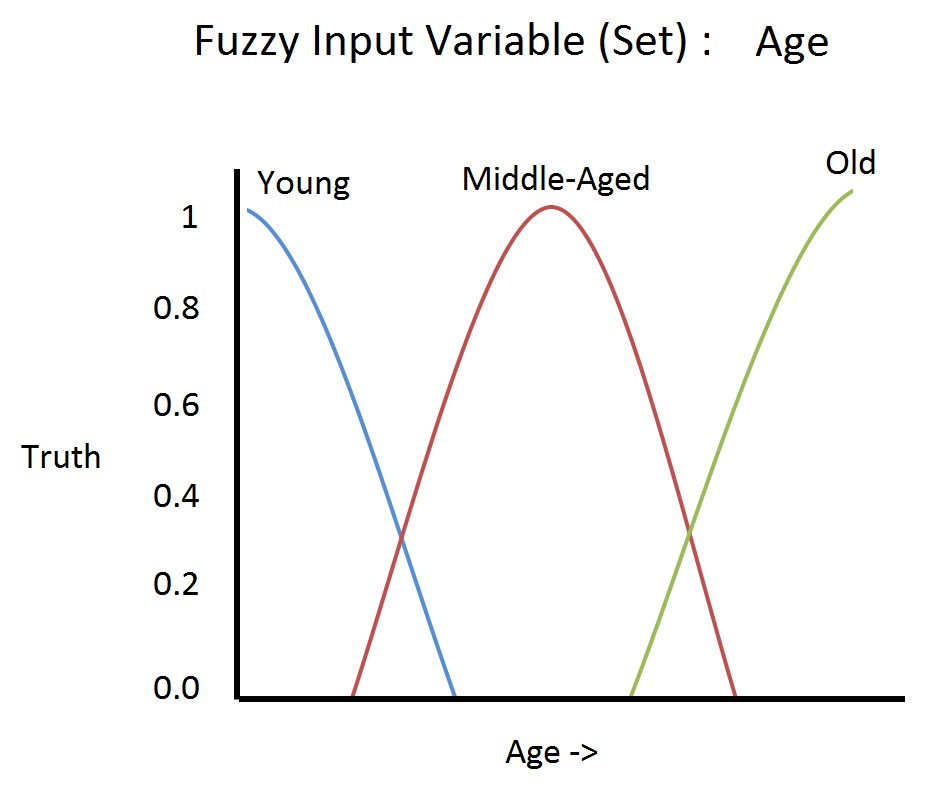
\includegraphics[width=0.6\textwidth]{images/Picture7.png}
	\end{figure}
\end{frame}

\begin{frame}
	\frametitle{Fuzzy Membership Functions}
	\begin{figure}[c]
	 \ \\
		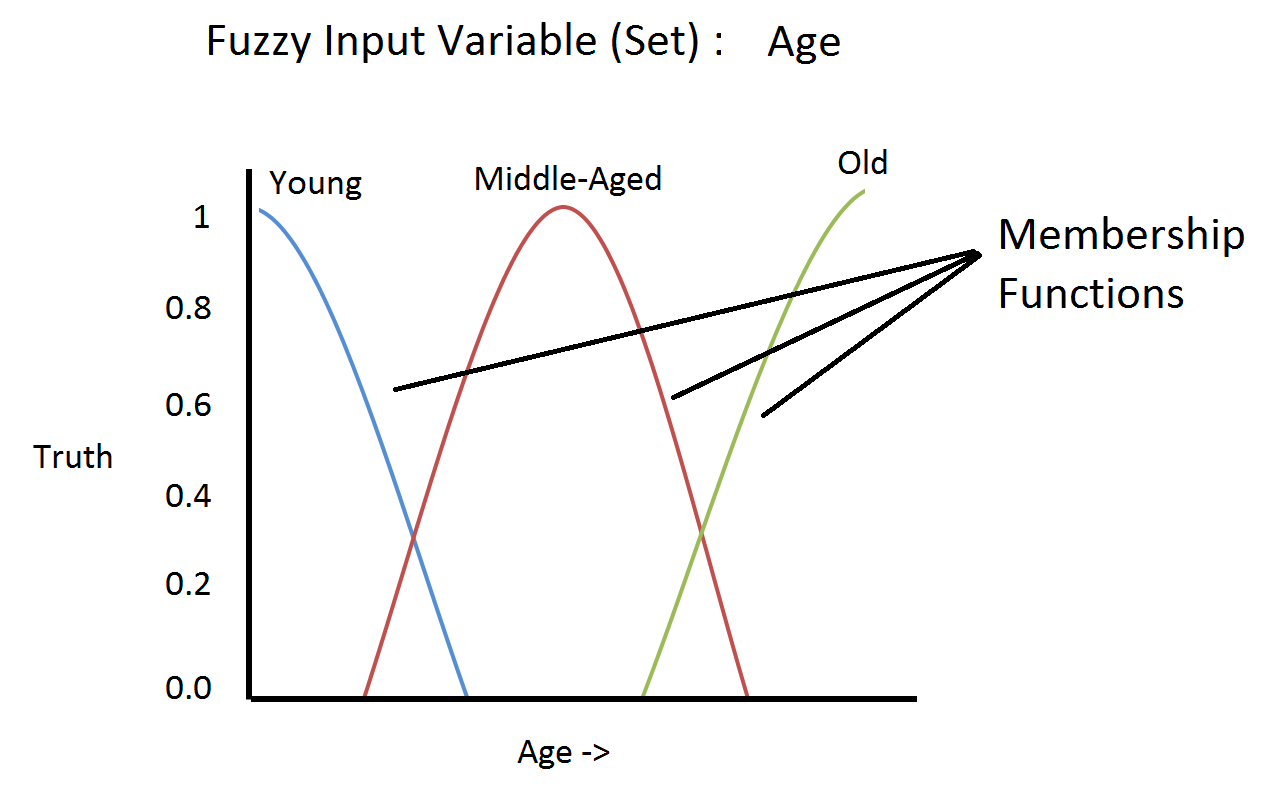
\includegraphics[width=0.75\textwidth]{images/Picture8.png}
	\end{figure}
\end{frame}




\begin{frame}
  \frametitle{Similar Systems}
		\pause
		\begin{itemize}
		\item MATLAB Fuzzy Toolbox
		\pause
		\item R Package, FuzzyToolkitUoN
		\pause
		\item X Fuzzy 3.0
		\pause
		\item \emph{fuzzy}TECH
		\end{itemize}
\end{frame}


\begin{frame}
\frametitle{What's wrong with them?}

\begin{itemize}
\pause
		\item Difficult to access
				\pause
				\begin{itemize}
				\item Finding them \pause
				\item Downloading/Installation \pause
				\item Cost \pause
				\end{itemize} 
		\item Difficult to use \pause
			\begin{itemize}
			\item Unintuitive interface - command line\pause
			\item Poorly maintained \pause
			\item Require too much prior knowledge
			\end{itemize}
		\end{itemize}
\end{frame}



\begin{frame}
 \frametitle{The Solution}
My plan: 
\pause
\emph{Web-based} system for creating and manipulating fuzzy systems. 
\pause
\ \\
\ \\
Incorporating the best features from existing systems
\pause
	  \begin{itemize}
	  	\item{Easy To Access}
	  	\pause
	  	\begin{itemize}
			\item Online   	  	\pause
			\item Can work with/produce a variety of file types 	  	\pause
		\end{itemize} 
		\item{Easy To Use} 	  	\pause
	  	\begin{itemize}				  
	  		\item Intuitive Design 	  	\pause
  			\item Unrestricted navigation \pause
	  		\item Dedicated un-interruptive help system 	  	\pause
	  		\item Abide by HCI principles 	  	\pause
		\end{itemize}
		\item{Extensibility} 	  	\pause
	  	\begin{itemize}				  		
	  		% When I spoke about using the best parts about existing systems....
	  		\item FuzzyToolkitUoN backend 
	  		\pause
	  		\item Directly use R commands
	  	\end{itemize}
	  \end{itemize}
\end{frame}


\begin{frame}
	\frametitle{The System Architecture}
	\begin{center}
	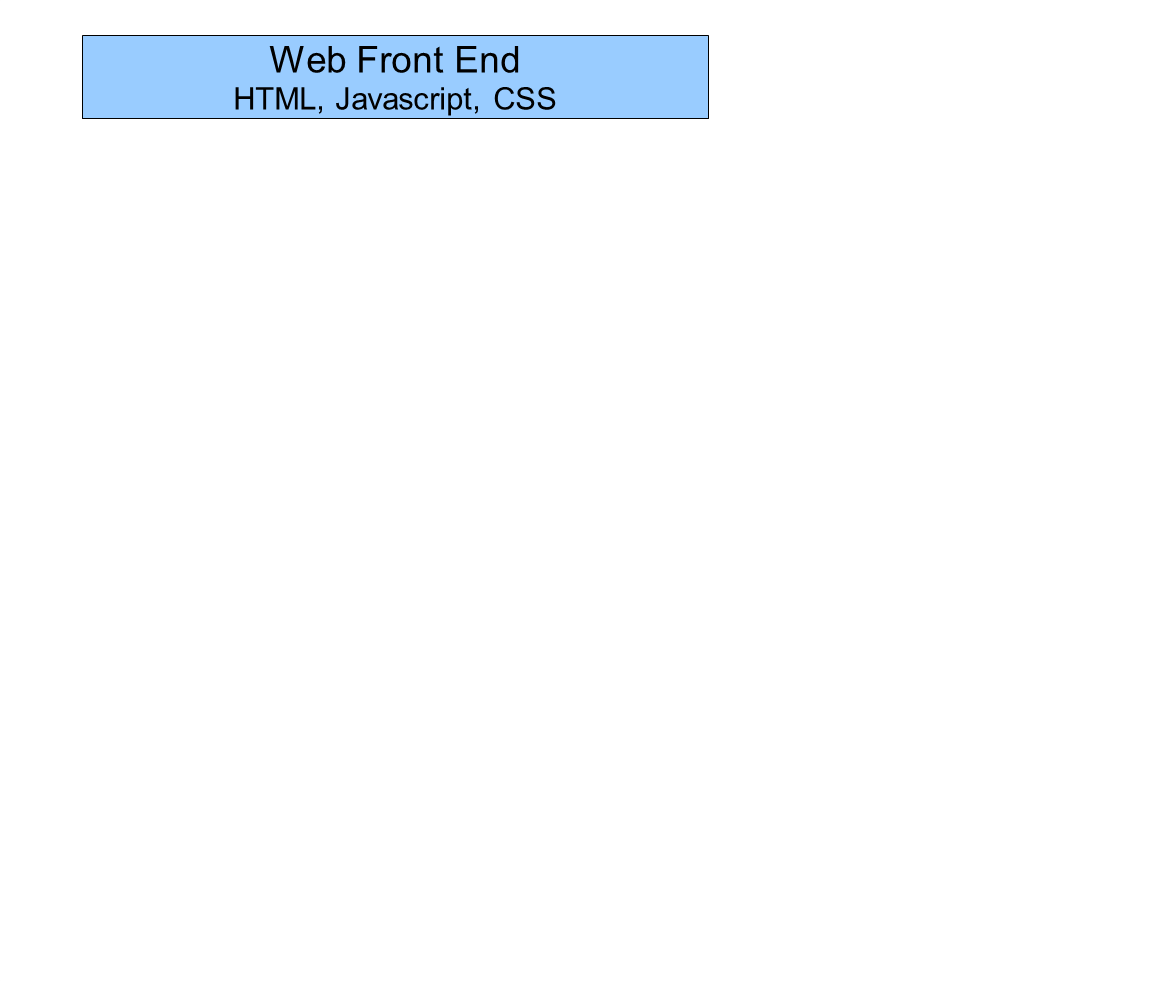
\includegraphics[width=0.75\textwidth]{images/Picture1.png}
	\end{center}
\end{frame}
\begin{frame}
	\frametitle{The System Architecture}
	\begin{center}
	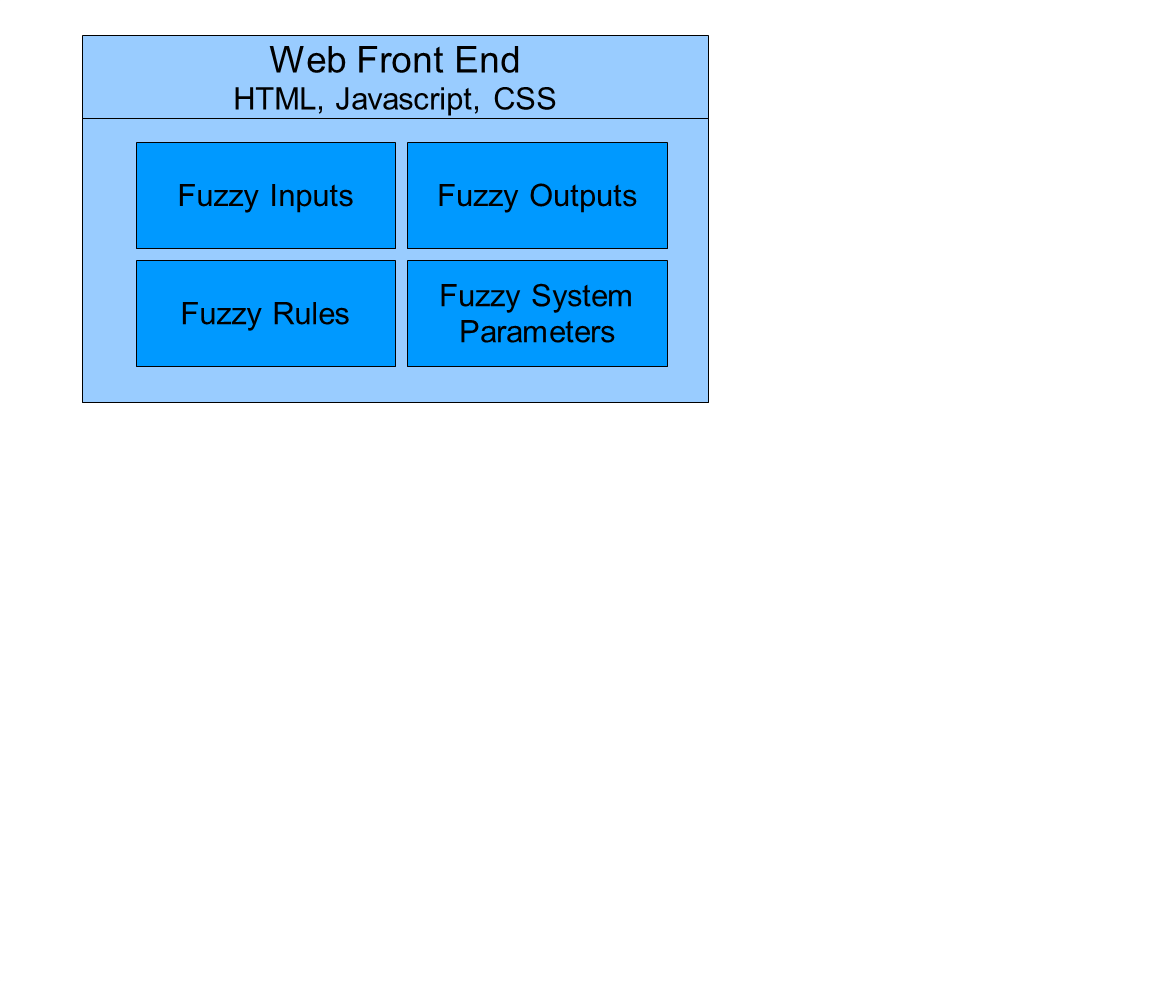
\includegraphics[width=0.75\textwidth]{images/Picture2.png}
	\end{center}
\end{frame}
\begin{frame}
	\frametitle{The System Architecture}
	\begin{center}
	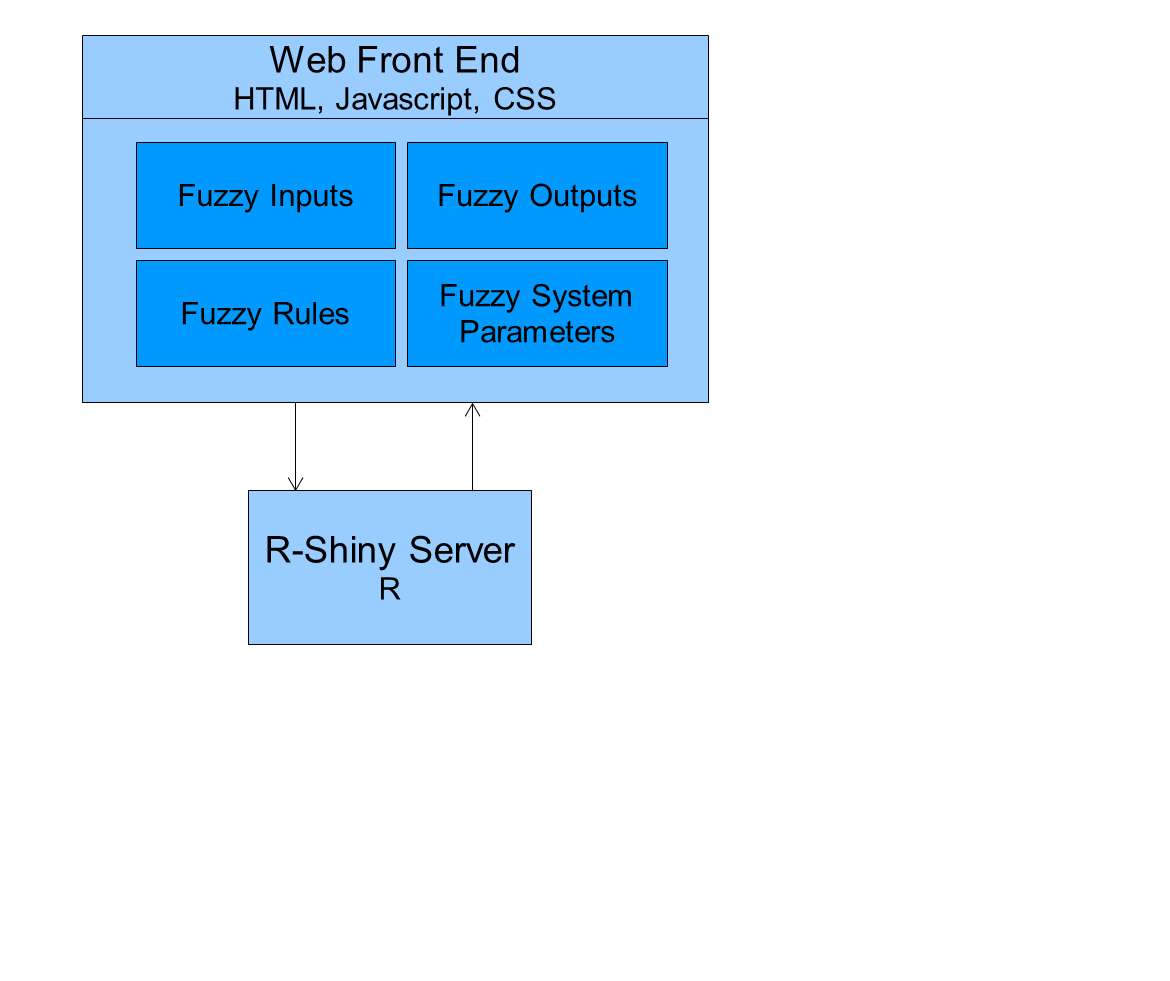
\includegraphics[width=0.75\textwidth]{images/Picture3.png}
	\end{center}
\end{frame}
\begin{frame}
	\frametitle{The System Architecture}
	\begin{center}
	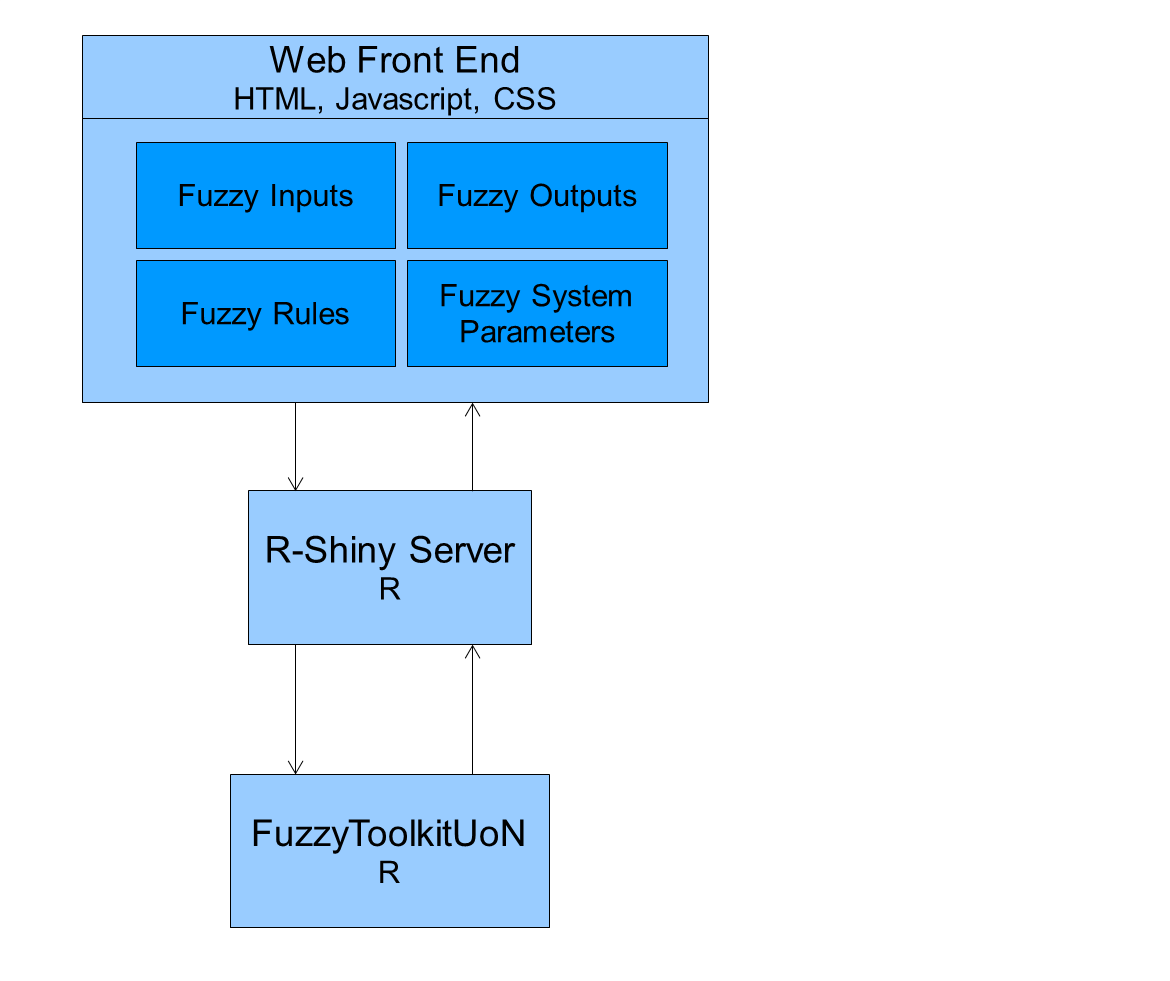
\includegraphics[width=0.75\textwidth]{images/Picture4.png}
	\end{center}
\end{frame}
\begin{frame}
	\frametitle{The System Architecture}
	\begin{center}
	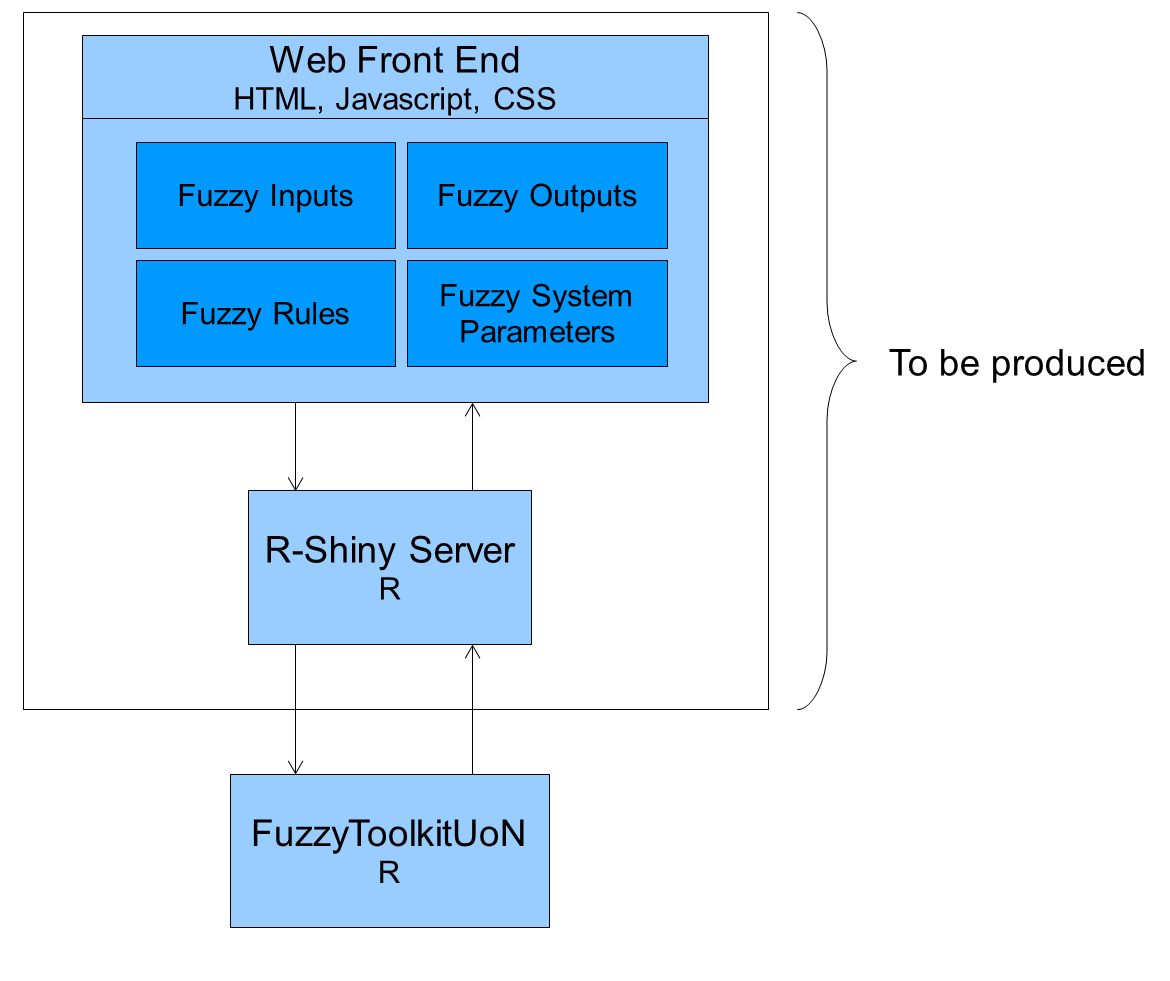
\includegraphics[width=0.75\textwidth]{images/Picture5.png}
	\end{center}
\end{frame}
\begin{frame}
	\frametitle{The System Architecture}
	\begin{center}
	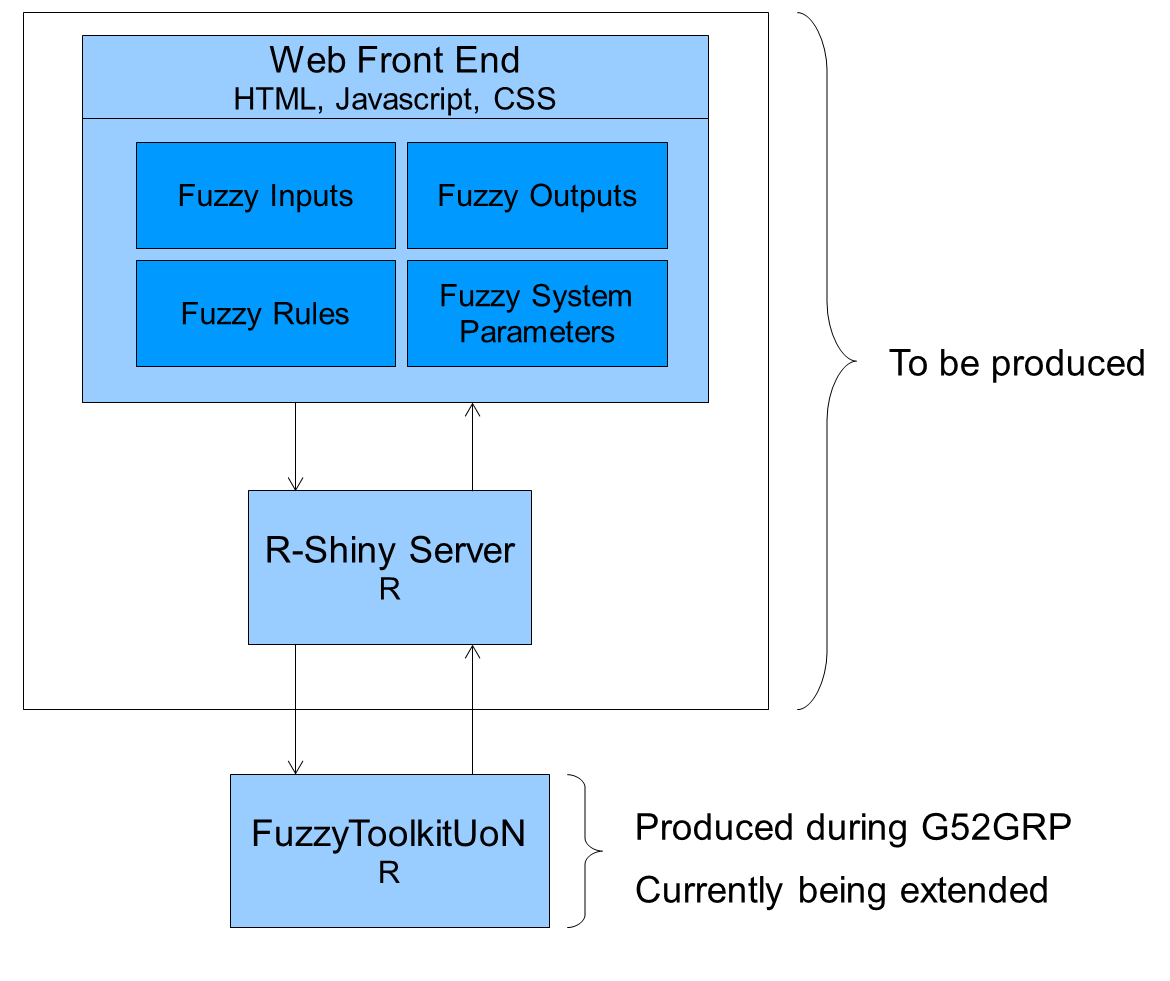
\includegraphics[width=0.75\textwidth]{images/Picture6.png}
	\end{center}
\end{frame}

\begin{frame}
 \frametitle{Proposed Progress}
 \begin{center}
 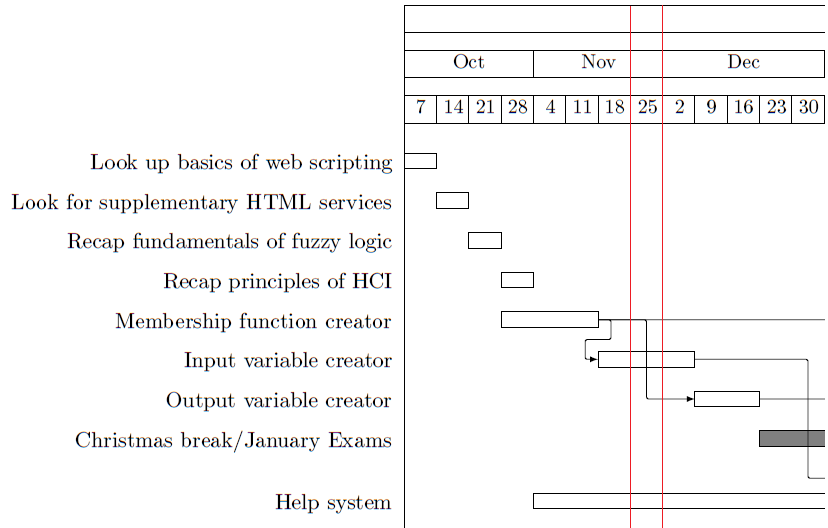
\includegraphics[width=0.9\textwidth]{images/GANTTONE.png}
 \end{center}
\end{frame}

\begin{frame}
 \frametitle{Progress (1)}
 \begin{mdframed}
 \begin{center}
 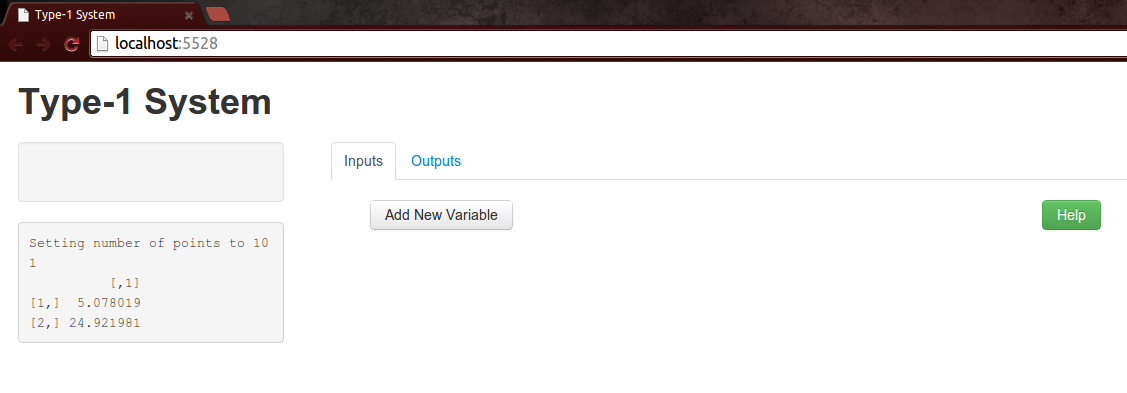
\includegraphics[width=0.9\textwidth]{images/fuz4.png}
 \end{center} 
 \end{mdframed}
\end{frame}
\begin{frame}
 \frametitle{Progress (2)}
 \begin{mdframed}
 \begin{center}
 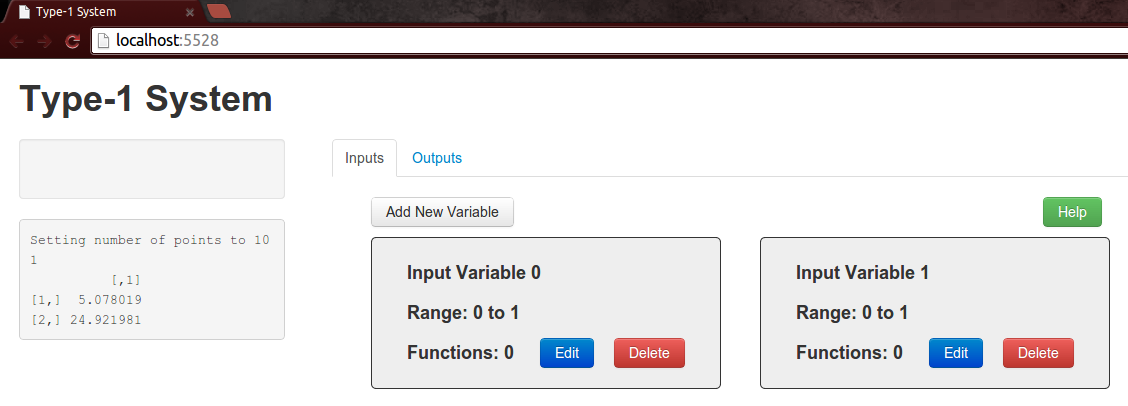
\includegraphics[width=0.9\textwidth]{images/fuz5.png}
 \end{center} 
 \end{mdframed}
\end{frame}
\begin{frame}
 \frametitle{Progress (3)}
 \begin{mdframed}
 \begin{center}
 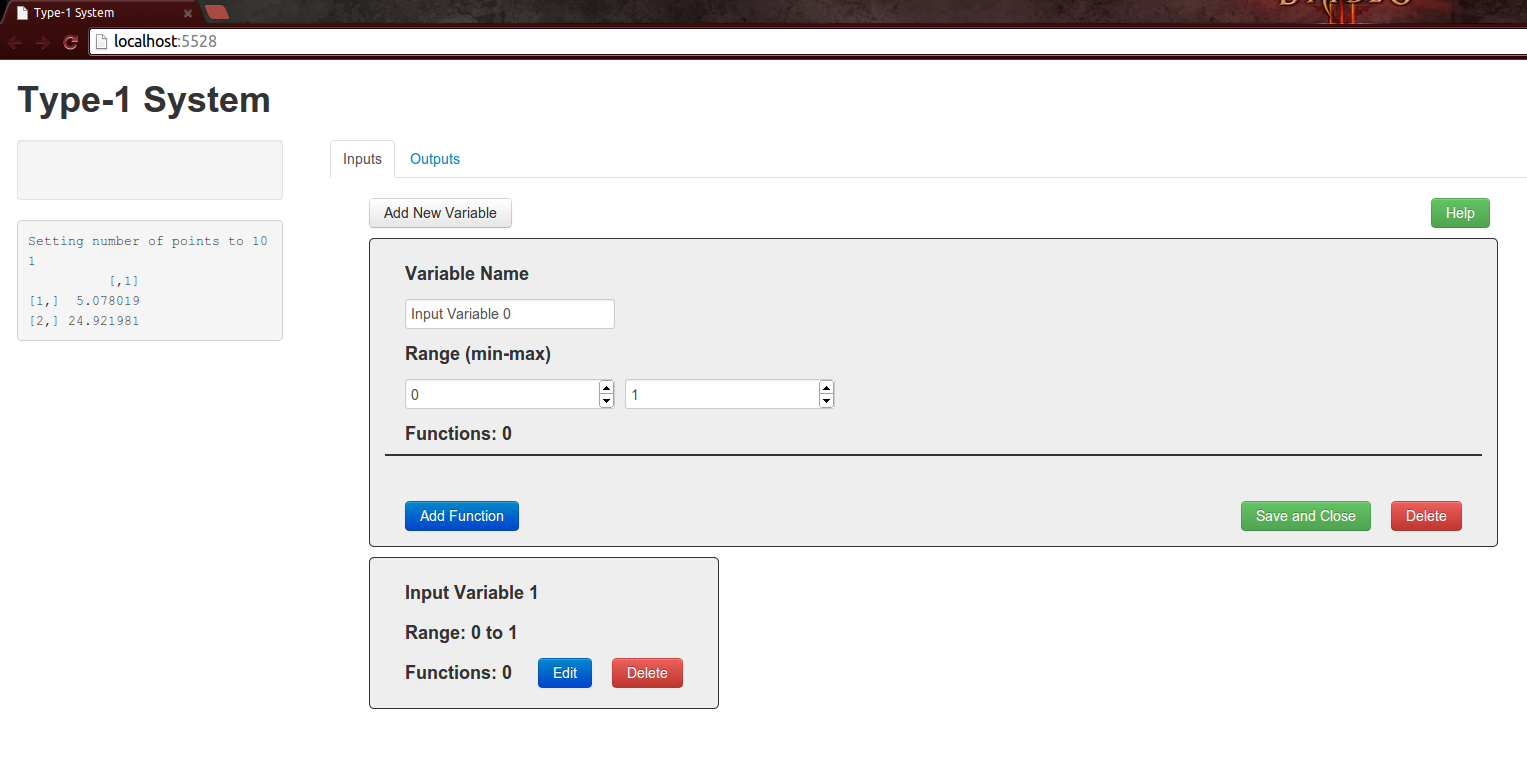
\includegraphics[width=0.9\textwidth]{images/fuz6.png}
 \end{center} 
 \end{mdframed}
\end{frame}
\begin{frame}
 \frametitle{Progress (5)}
 \begin{mdframed}
 \begin{center}
 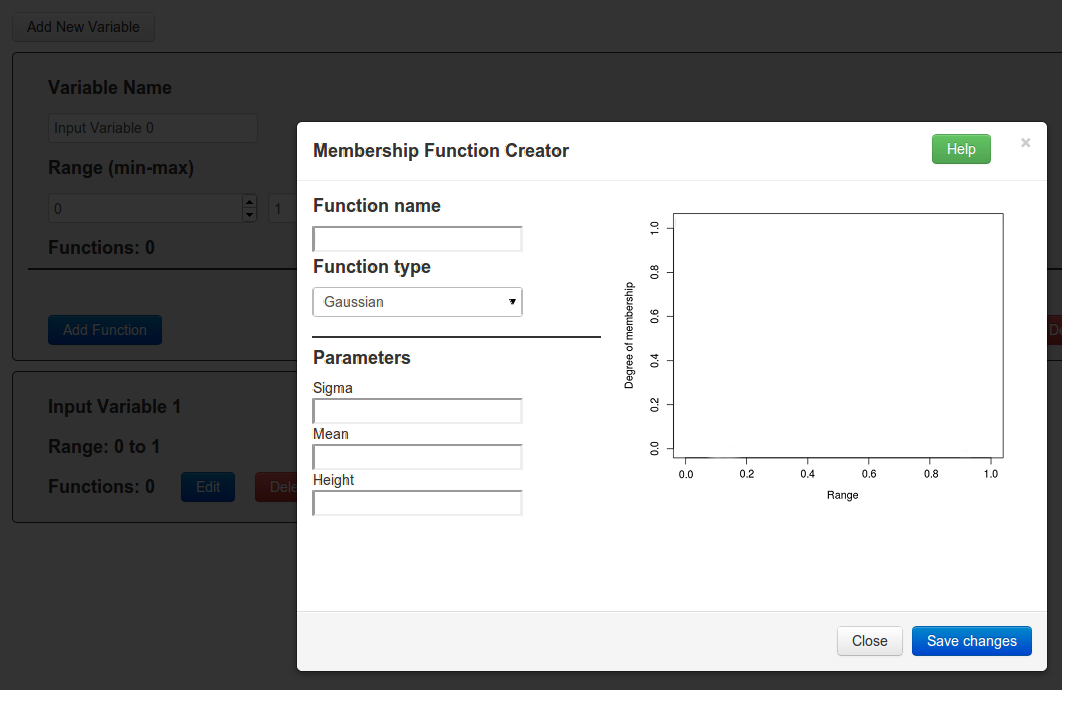
\includegraphics[width=0.9\textwidth]{images/fuz8.png}
 \end{center} 
 \end{mdframed}
\end{frame}
\begin{frame}
 \frametitle{Progress (6)}
 \begin{mdframed}
 \begin{center}
 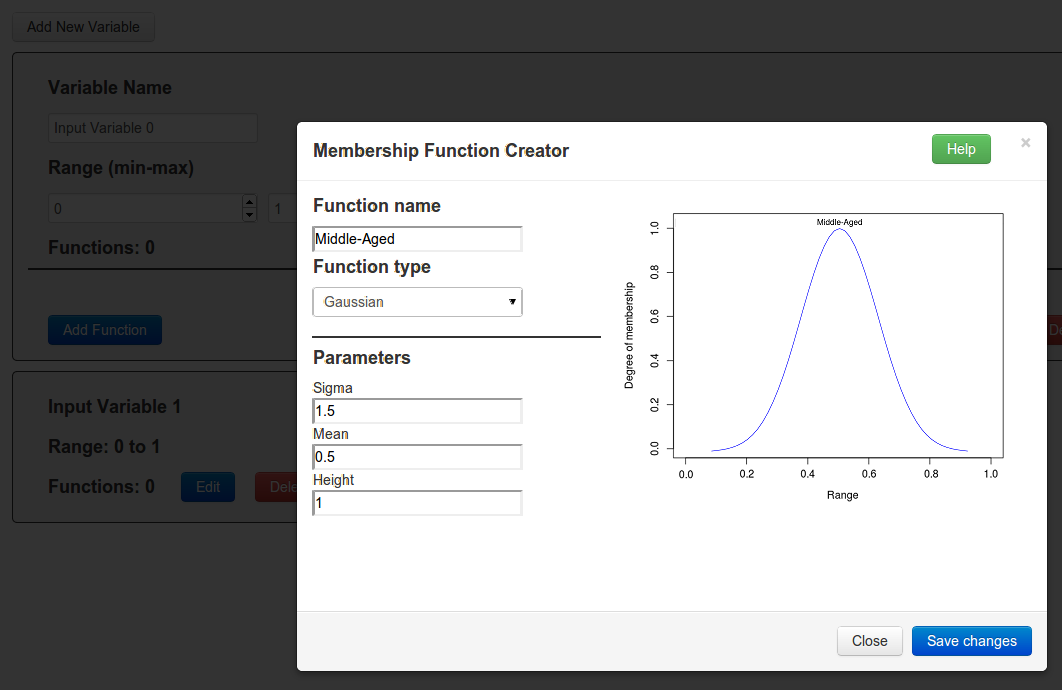
\includegraphics[width=0.85\textwidth]{images/fuz9.png}
 \end{center} 
 \end{mdframed}
\end{frame}

\begin{frame}
 \frametitle{Progress (8)}
 \begin{mdframed}
 \begin{center}
 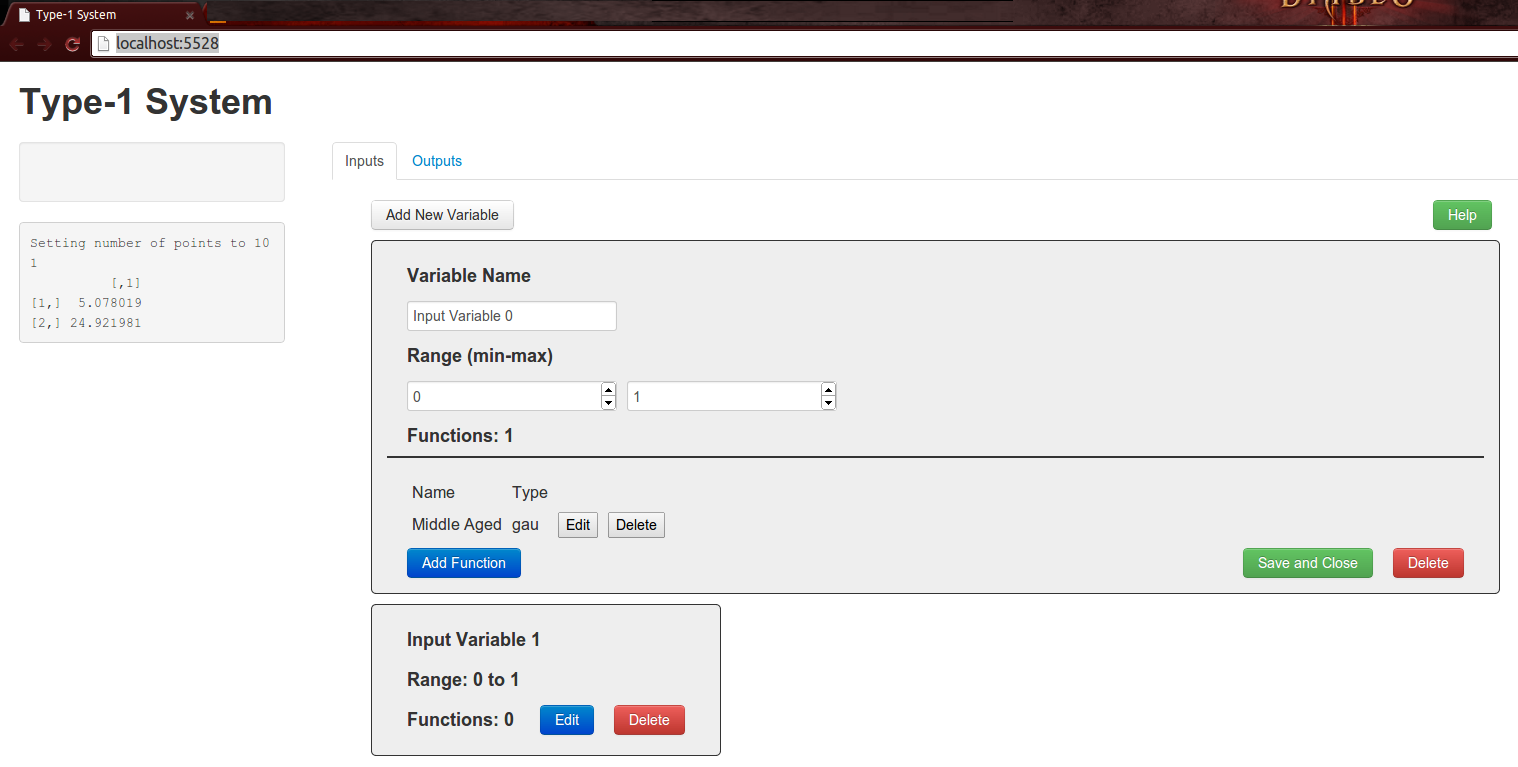
\includegraphics[width=0.85\textwidth]{images/fuz10.png}
 \end{center} 
 \end{mdframed}
\end{frame}


\title{Fuzzy Logic}
\begin{frame}
 \frametitle{Actual Progress}
 \begin{center}
 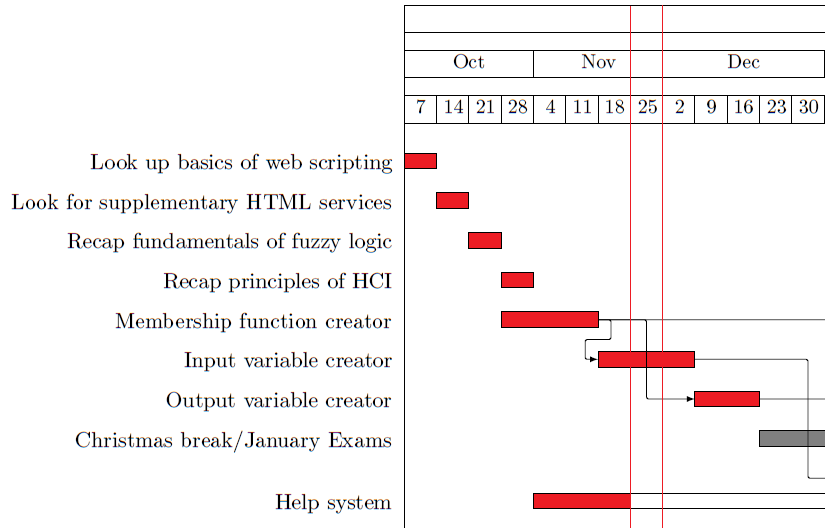
\includegraphics[width=0.9\textwidth]{images/GANTTTWO.png}
 \end{center}
\end{frame}

\begin{frame}
 \frametitle{Extended Progress}
 \begin{mdframed}
 \begin{center}
 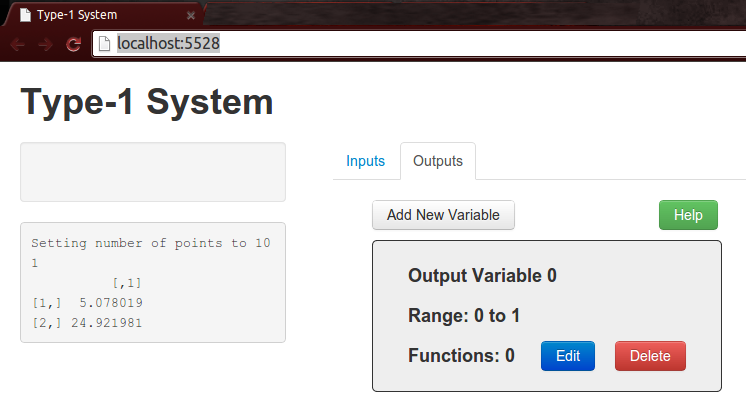
\includegraphics[width=0.85\textwidth]{images/fuz11b.png}
 \end{center} 
 \end{mdframed}
\end{frame}

\title{Fuzzy Logic}
\begin{frame}
 \frametitle{Questions?}
 \begin{center}
  Web Based Fuzzy Inferencing and Visualisation.\ \\
 Craig Knott\ \\

 \ \\
 Any Questions?
 \end{center}
\end{frame}


\end{document}